%************************************************
\chapter{Case Study}\label{ch:case_study}
%************************************************
Part of the evaluation of the developed tool is to verify the functionality with an industrial company. In order to do so, a company closely related to the University of Groningen has been found. This company is named `Sustainable Buildings' and sells products to monitor the users electricity and gas consumption in real-time. This leads to an increase in building-users awareness by providing real-time feedback through public dashboards \cite{sb}.\\

\noindent
In order to serve their customers, they have allocated a physical server consisting of 40 cores and 128 GB of RAM. Additionally, they have 900 GB of storage data. This host machine is divided into 6 virtual machines. A brief overview of their architecture is described in \autoref{sec:sb-architecture}. This company perfectly meets the requirements for evaluating the tool, because it is a relatively large system with many load. Additionally, the tool might be useful for them, as they are now missing insights into their performance. The process of deploying this system has been described in \autoref{sec:sb-process}. At the end, an evaluation has been performed. This evaluation consists of an interview and is described in \autoref{sec:sb-evaluation}.

\section{Architecture} \label{sec:sb-architecture}
The six virtual machines work together as one system. Each virtual machine is responsible for running a number of services. These services can be found in \autoref{fig:sb-architecture}. In order to simplify the deployment, the employees of the company decided to assign a name to every VM. The names are also presented in the architecture diagram. A small overview of the number of CPU, RAM and memory per VM can be found in \autoref{tab:vms}. As described in \autoref{sec:architecture}, the architecture consists of a single root-node, two super-nodes and three nodes. The structure can be found in \autoref{fig:sb-tree}. From this figure it becomes clear that Jotunheim consumes two roles. Both as a root, and as a supernode.


\begin{figure}
    \centering
    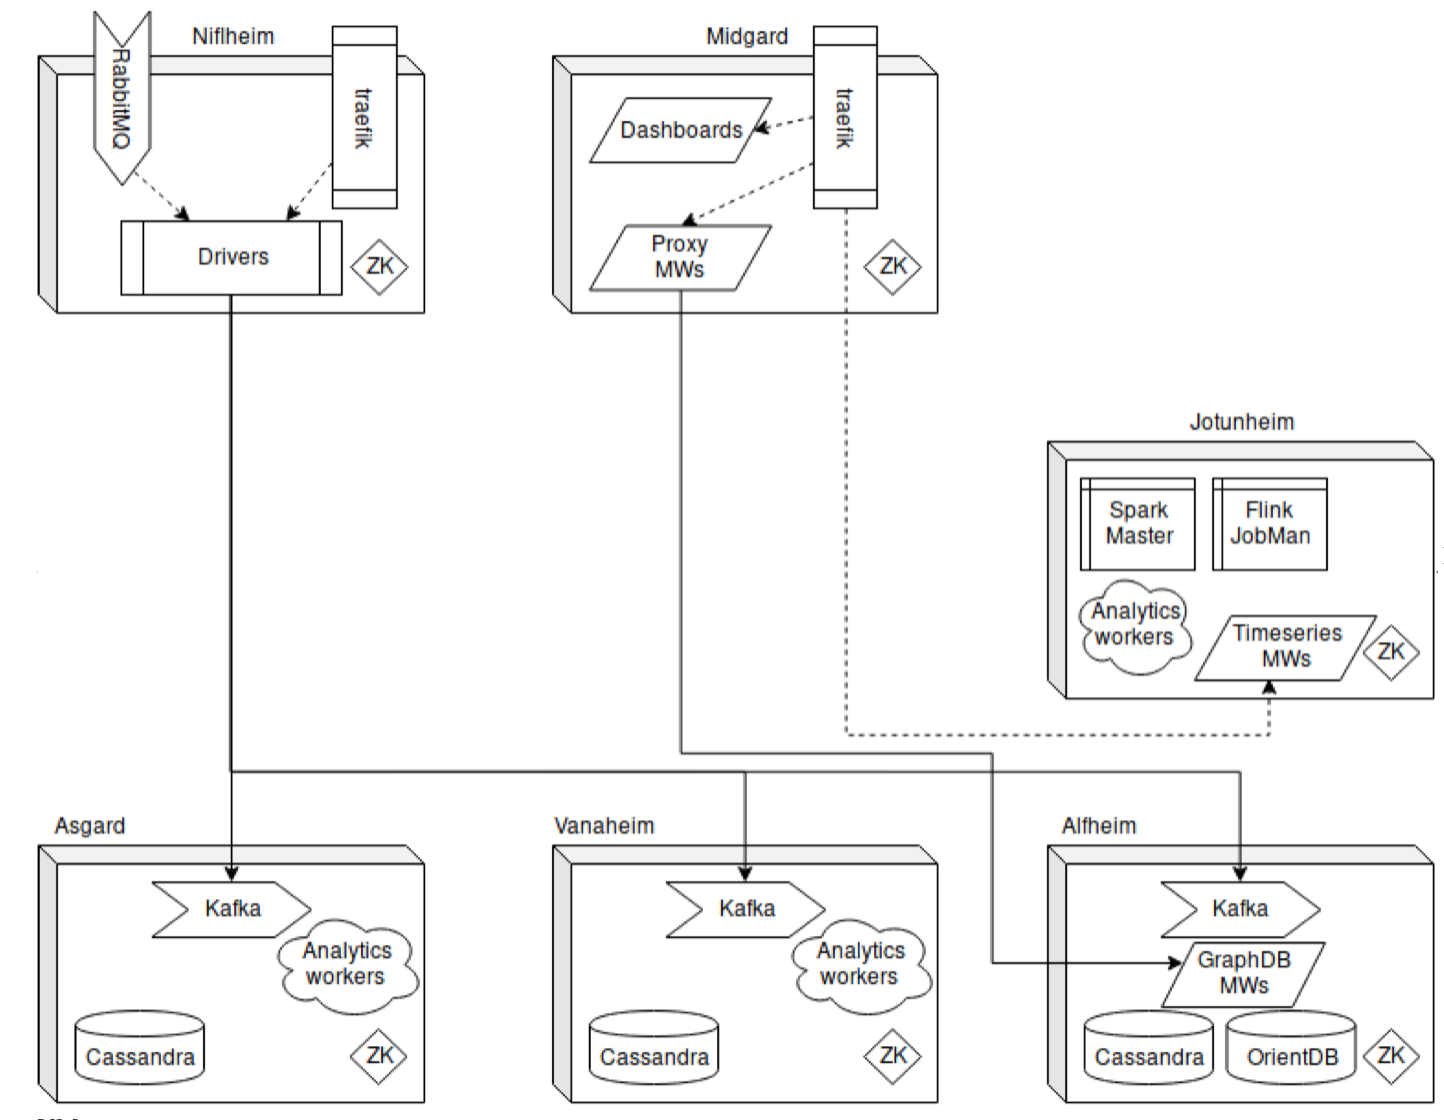
\includegraphics[width=\textwidth]{gfx/sb-architecture.png}
    \caption{Sustainable Buildings architecture}
    \label{fig:sb-architecture}
\end{figure}

\begin{table}
    \centering
    \begin{tabular}{l|lrrr}
        Virtual Machine &IP & Cores & RAM & Memory \\ \hline
        Asgard & 192.168.1.10 &8 & 16 GB & 100 GB \\
        Vanaheim & 192.168.1.11 &8 & 16 GB & 100 GB \\
        Alfheim & 192.168.1.12  &8 & 16 GB & 100 GB \\
        Jotunheim & 192.168.1.13 &8 & 16 GB & 100 GB \\
        Midgard & 192.168.1.14 &4 & 8 GB & 20 GB \\
        Niflheim & 192.168.1.15 &4 & 8 GB & 20 GB \\
    \end{tabular}
    \caption{Overview of the architecture}
    \label{tab:vms}
\end{table}

\begin{figure}
    \centering
    \begin{forest}
        for tree={
            grow=south,
            rectangle, draw, minimum size=3ex, inner sep=1pt,s sep=7mm
        }
        [~~Jotunheim~~~ 
        [~~Vanaheim~~~ 
          [~~Asgard~~~]
          [~~Alfheim~~~]
        ]
        [~~Jotunheim~~~
          [~~Midgard~~~]
          [~~Niffelheim~~~]
        ]
        ]
    \end{forest}
    \caption{Hierarchical overview of the Case study}
    \label{fig:sb-tree}
\end{figure}

\section{Deployment process} \label{sec:sb-process}
This section describes the process of deploying the implemented system on their architecture. This deployment has been made possible within three meetings. They are shortly described in the sub-sections below.

\subsection{First meeting}
Each meeting last around three hours. After the first meeting, there were several issues. Initially, the developed system was implemented in such a way that the nodes were communicating over their public IP address. However, it turned out that not every node was publicly accessible. Therefore, the program was updated, such that they communicate over their internal IP. Another issue was due to the amount of load going in and out their system. Therefore, the part of the program that monitors the internet traffic with respect to the containers raised its CPU to above 100\% as can be seen in \autoref{fig:100}.
The decision was therefore made to not deploy the program any more, and first solve the issues that showed up.

\begin{figure}
    \centering
    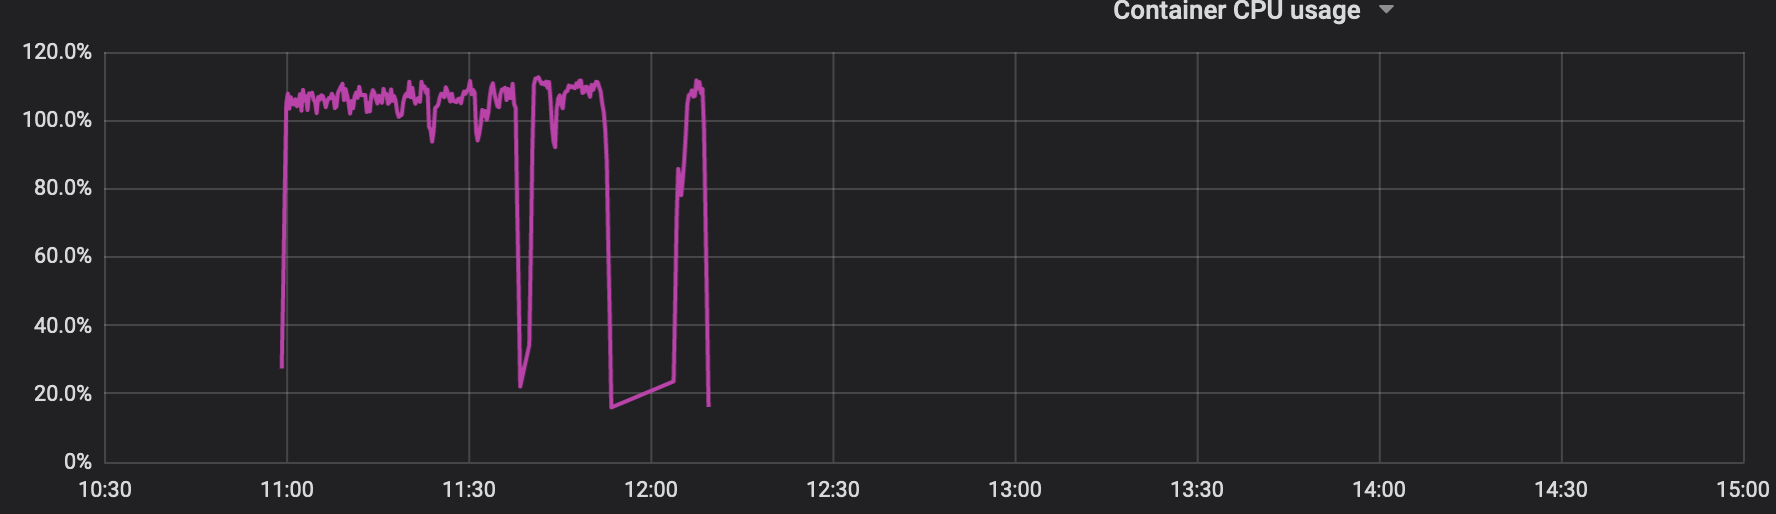
\includegraphics[width=\textwidth]{gfx/load-100.png}
    \caption{CPU data of the deployed system during the first meeting}
    \label{fig:100}
\end{figure}

\subsection{Second meeting}
In order to solve the issue described in the previous sub-section, a sub sampling of the internet monitoring was applied. Therefore, instead of capturing all packets, the packets where captured for $x$ seconds, while sleeping $y$ seconds. However, for every packet that is coming from a peer within the system, the program tries to assign this packet directly to a remote Docker container. Therefore, there was still a significant amount of communication overhead, which can be seen in \autoref{fig:60}. Eventually, the program kept growing CPU resources consumed, which lead to the conclusion that the program was not efficient enough. Therefore, the program was not deployed.

\begin{figure}
    \centering
    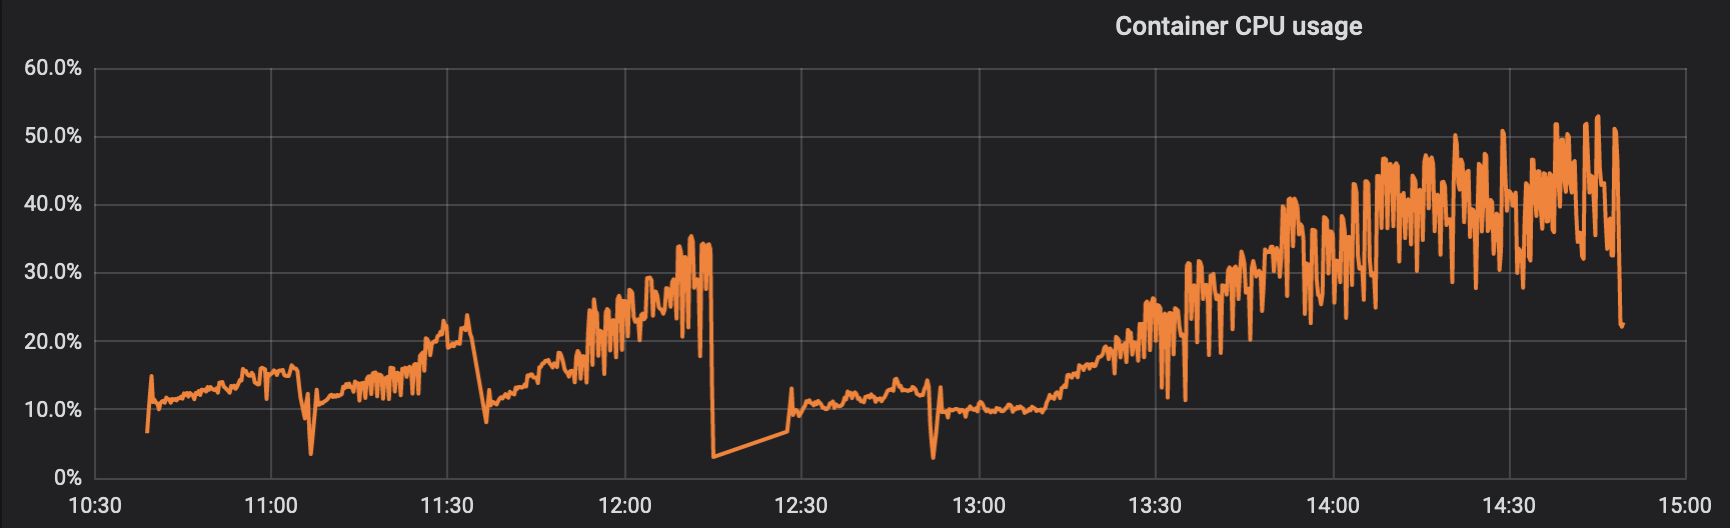
\includegraphics[width=\textwidth]{gfx/load-60.png}
    \caption{CPU data of the deployed system during the second meeting}
    \label{fig:60}
\end{figure}

\begin{figure}
    \subfloat[Asgard]{%
        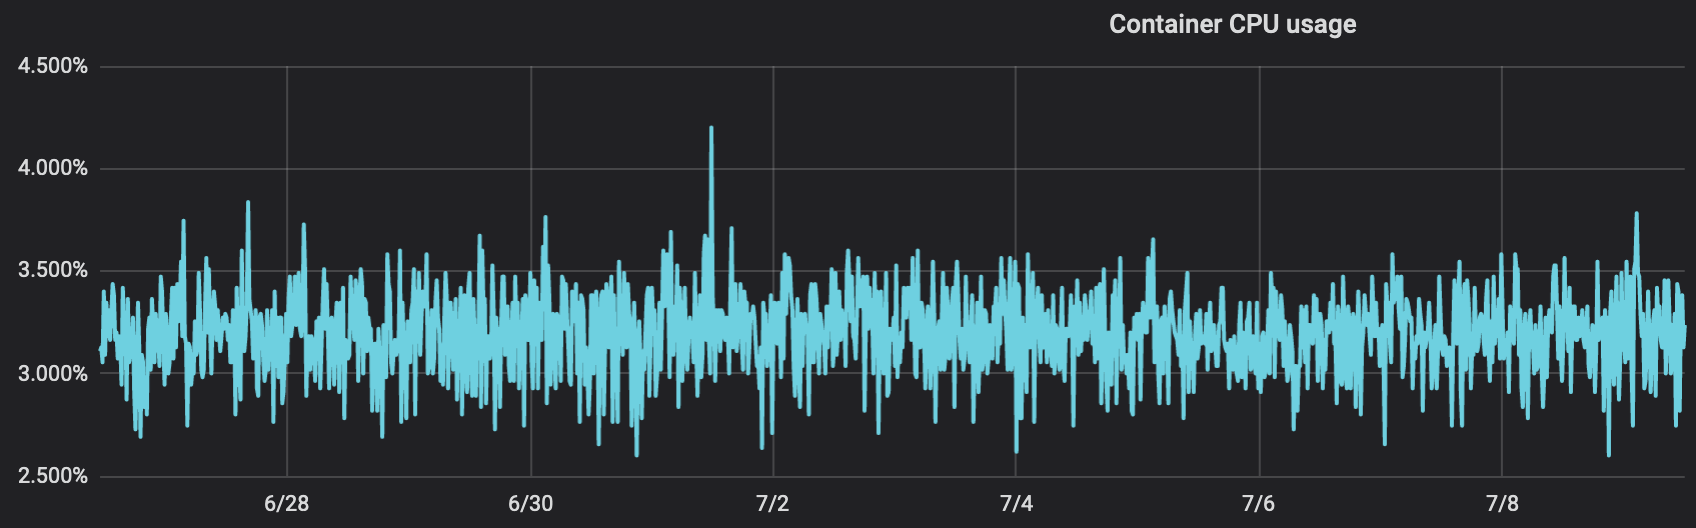
\includegraphics[width=0.45\textwidth]{gfx/asgard.png}
        \label{fig:deployment:asgard}
    }\qquad
    \subfloat[Midgard]{
        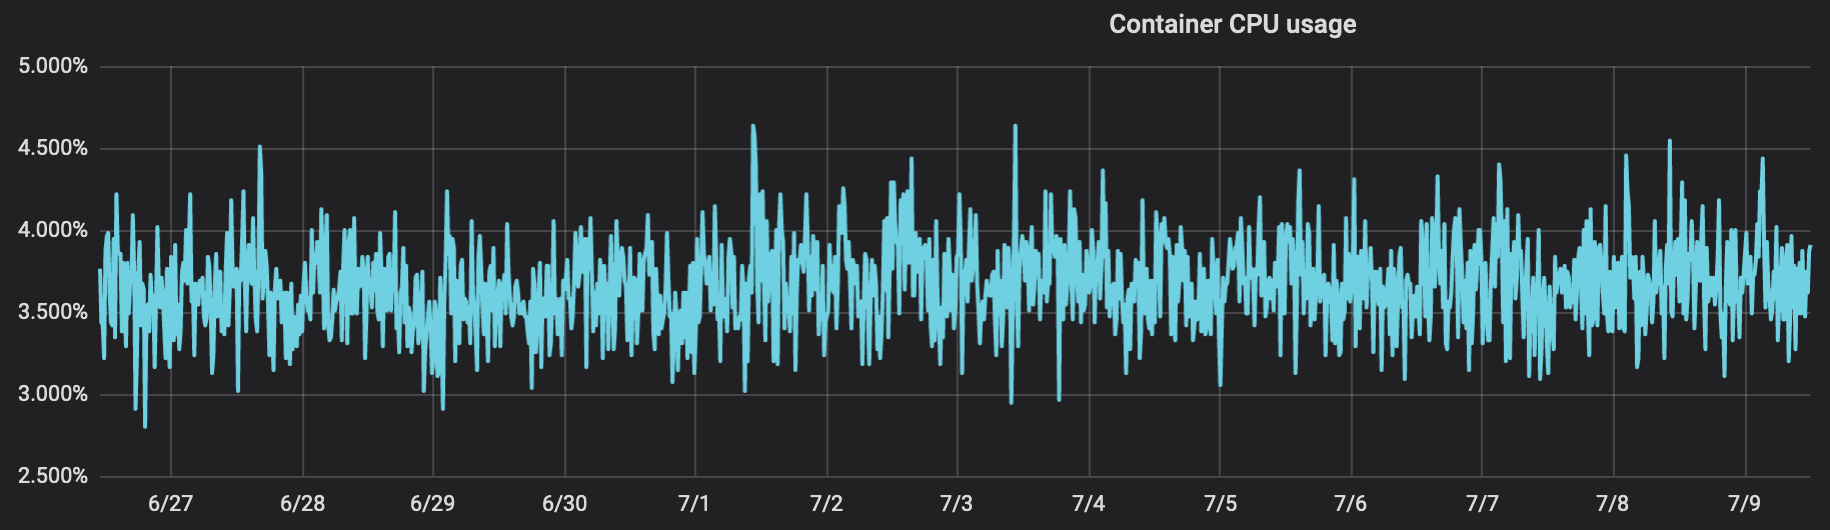
\includegraphics[width=0.45\textwidth]{gfx/midgard.png}%
        \label{fig:deployment:midgard}
    }
    
    \subfloat[Vanaheim]{%
        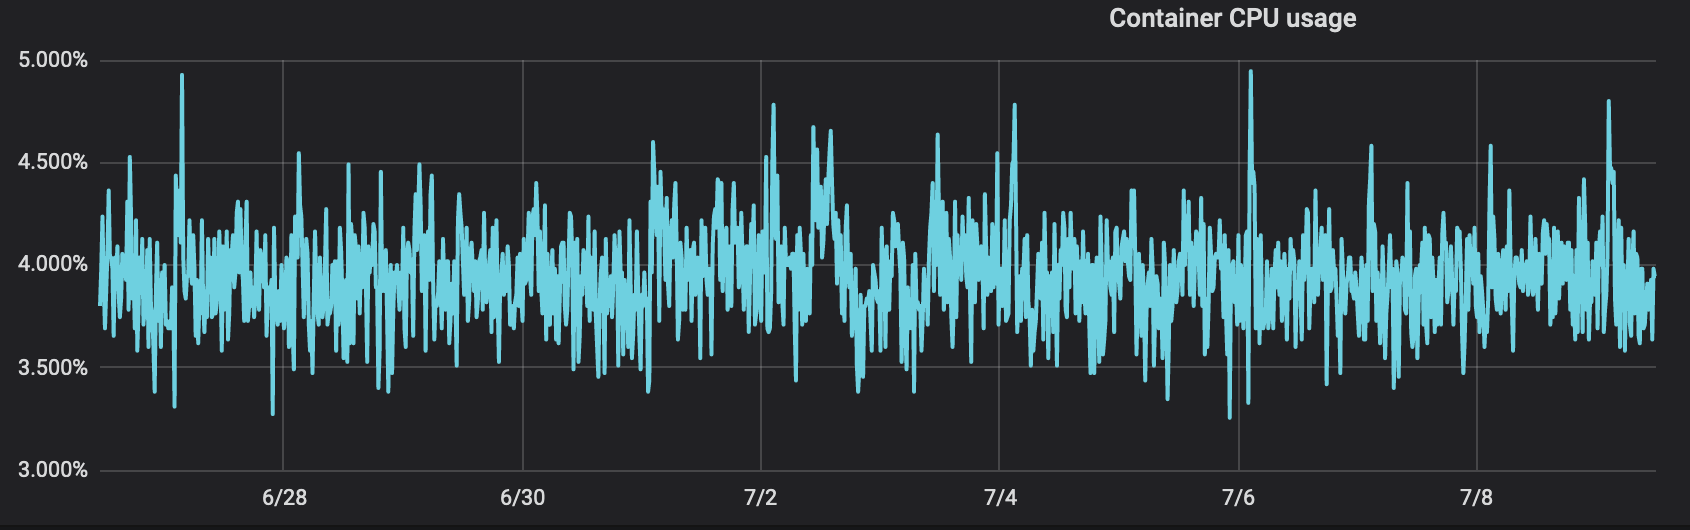
\includegraphics[width=0.45\textwidth]{gfx/vanaheim.png}
        \label{fig:deployment:vanaheim}
    }\qquad
    \subfloat[Alfheim]{
        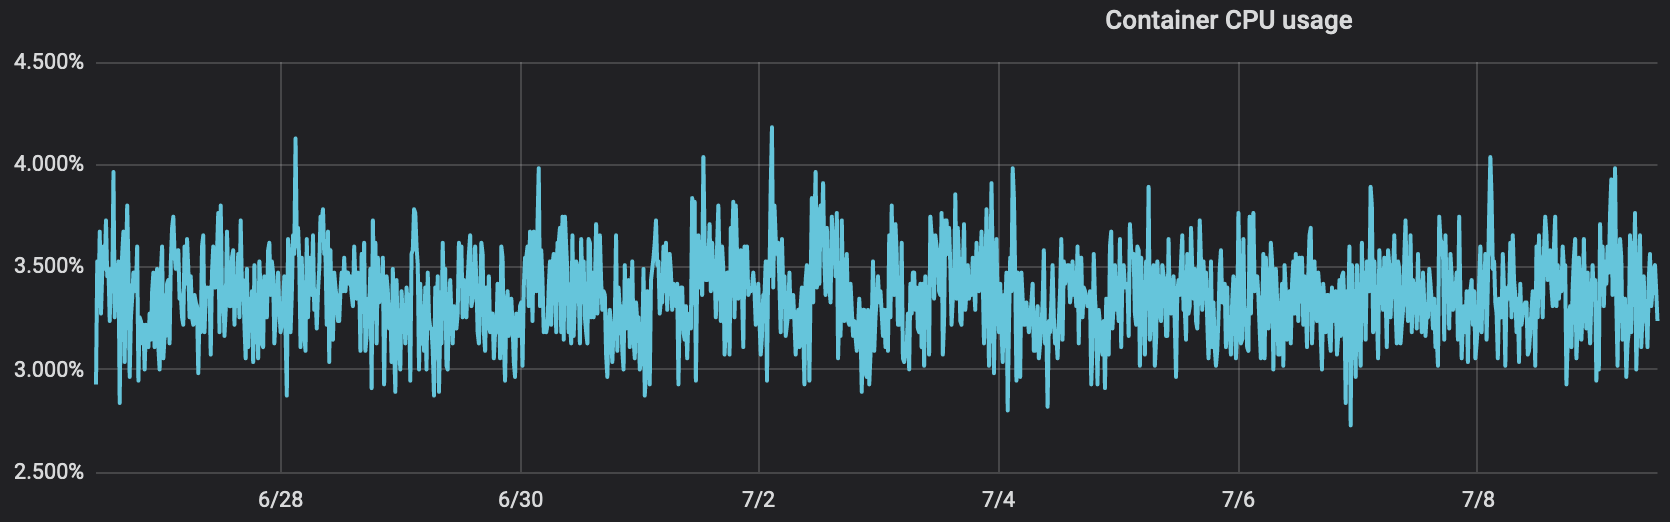
\includegraphics[width=0.45\textwidth]{gfx/alfheim.png}%
        \label{fig:deployment:alfheim}
    }
    
    \subfloat[Jotunheim]{%
        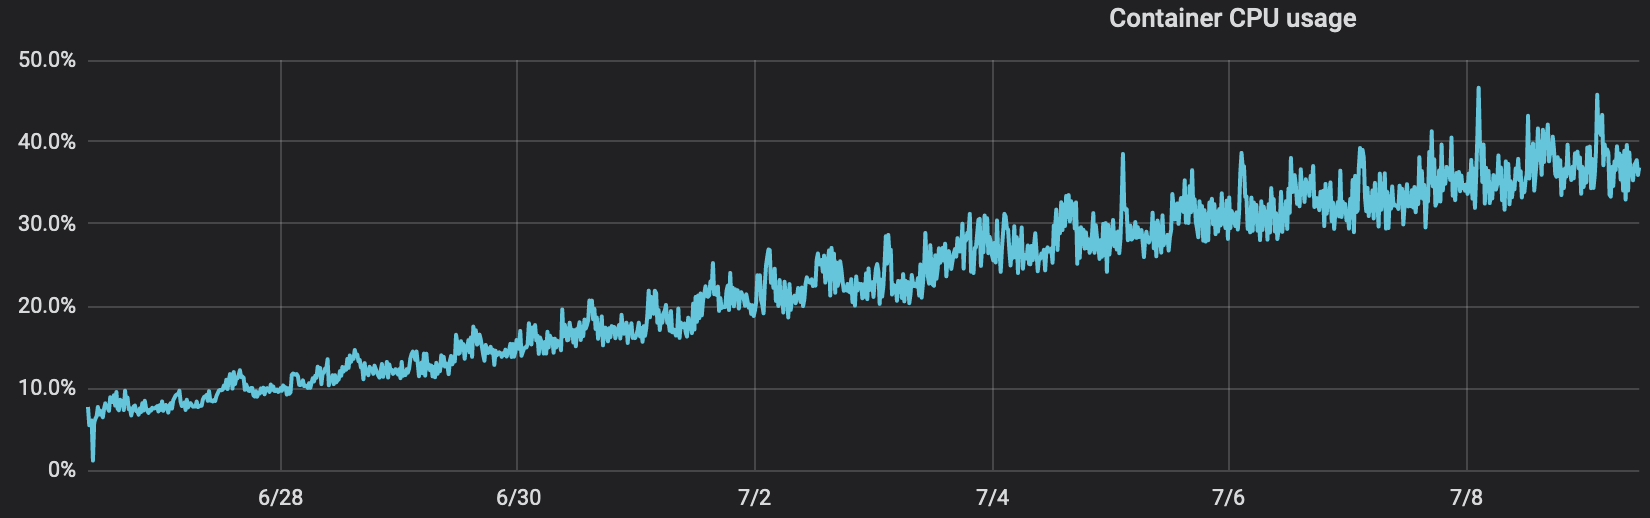
\includegraphics[width=0.45\textwidth]{gfx/jotunheim.png}
        \label{fig:deployment:jotunheim}
    }\qquad
    \subfloat[Niflheim]{
        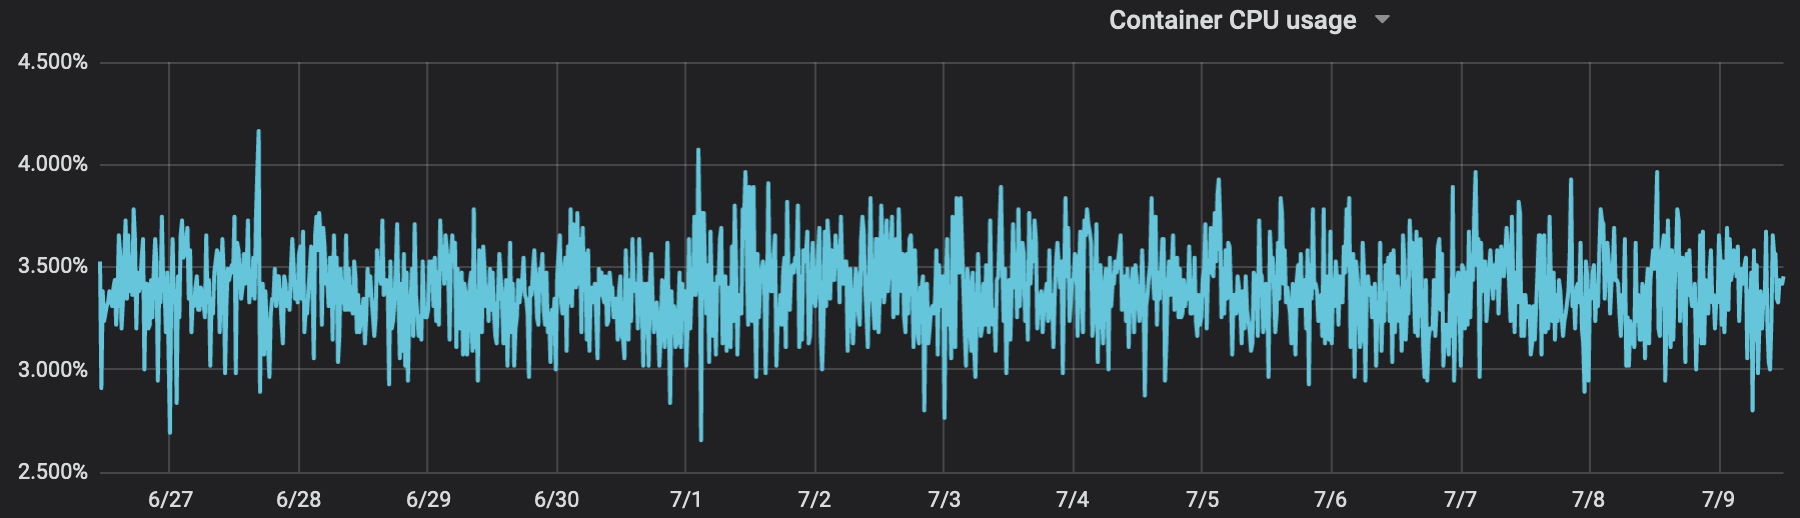
\includegraphics[width=0.45\textwidth]{gfx/niflheim.png}%
        \label{fig:deployment:niflheim}
    }
    
    \subfloat[Jotunheim Root]{%
        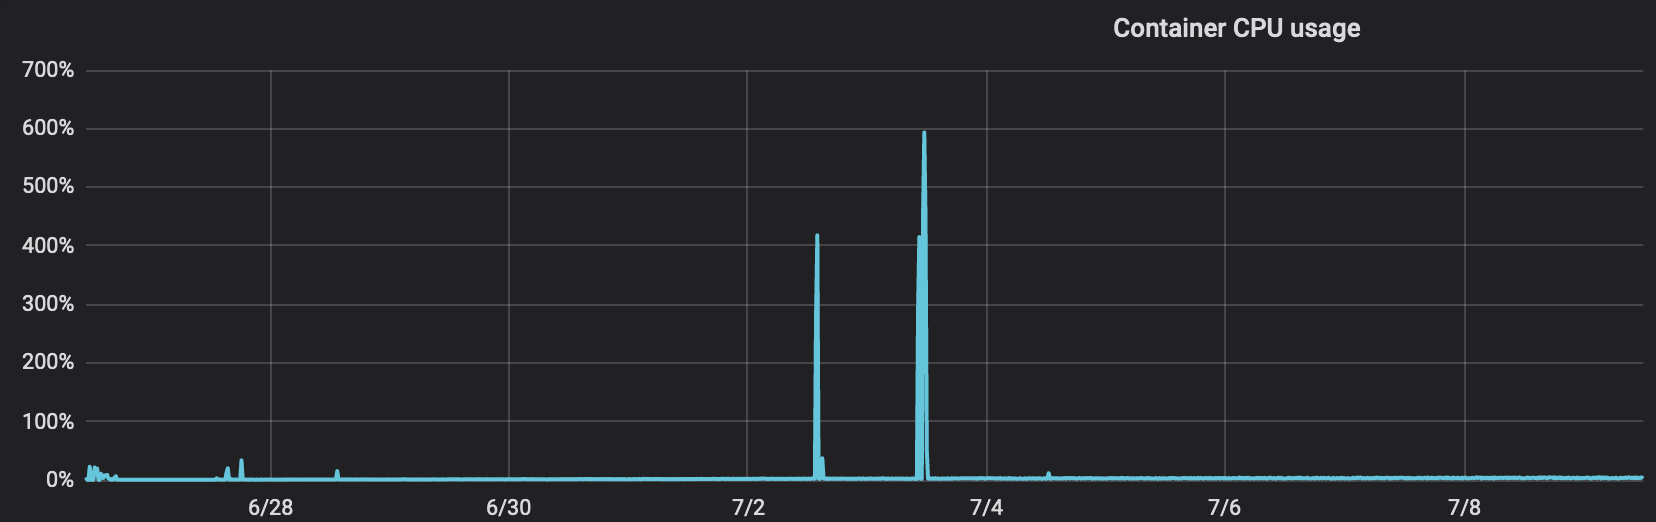
\includegraphics[width=0.45\textwidth]{gfx/jotunheim-root.png}
        \label{fig:deployment:jotunheim-root}
    }
    \caption{CPU utilization of the deployed system at 6 different VMs.}
    \label{fig:deployment}
\end{figure}

\subsection{Third meeting}
In order to solve the issue from the second meeting, the decision was made to implement a caching functionality. This means that the program resolves the internet traffic packets afterwards instead of real-time. The decision was made to implement a caching time limit of one minute, such that the obtained results are near real-time. The system therefore only communicates with its other nodes once per minute. This leads to a more efficient CPU usage, which can be seen in \autoref{fig:deployment}. This figure shows the CPU usage during the lifetime of the system. It can be concluded that the overall  CPU percentage is low, around 4\% for the nodes, and the root. However, for an unknown reason, the Jotunheim supernode linearly grows until 40\%, while the others stay constant. The Jotunheim root shows an average of 2.5\% CPU.

\section{Results}
In order to simply the results, several containers are grouped together using a regular expression. If a certain container name matches a regular expression, then this container is assigned to a certain group. The `other' group acts as a wildcard, matching every container that doesn't belong to a group. \autoref{tab:regex} shows the groups that are proposed, as well as the number of containers in this group.\\

\begin{table}
    \centering
    \begin{tabular}{l|lr}
        Regular expression & Group name & Containers \\ \hline
        / & other & 42 \\
        spark & sparkthings & 5\\
        flink & flinkthings & 4\\
        zookeeper & zookeeper & 5\\
        kafka & kafka & 11\\
        exporter & node-exporter & 5\\
        socat & socats & 6\\
        cassandra & cassandra & 3\\
        rest & timeseriest-rest & 3\\
        vault & vault & 6\\
        hadoop & hadoop & 4\\
        airflow & airflow & 3\\
        orchestrator & orchestrator & 2\\
        mw & middlewares & 12\\
    \end{tabular}
    \caption{Assigning container groups}
    \label{tab:regex}
\end{table}

\noindent
The services at the Sustainable Buildings Company have been monitored for exactly 14 days (from June 26, 11 AM UTC until July 10, 11 AM UTC). During these days, the resources have been monitored on a containerized level, and the waste cost is distributed over the running containers. The results of the cost and waste computation is summarized in \autoref{fig:stats}. This computation is based on the prices proposed in \autoref{sec:pricing}, except for the $p_\text{network}$. In \autoref{sec:sb-limitations}, it is described that the traffic monitoring has several limitations. Therefore, the network price has been updated to $p_\text{network} = 0.05$, which is half of the proposed pricing. This is based on the assumption that half of the network traffic is internal (between their services), and other half of the network traffic is external.\\

\begin{figure}
    \centering
    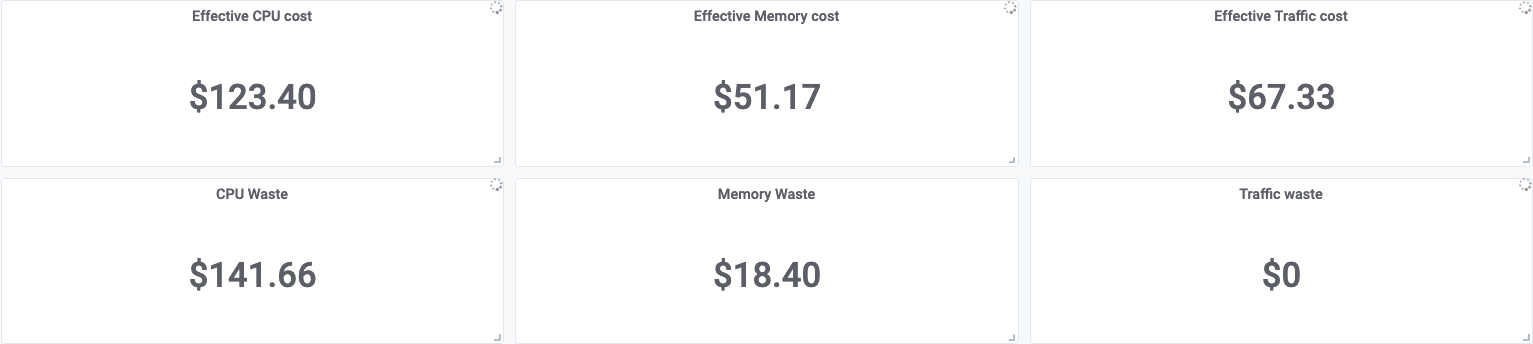
\includegraphics[width=\textwidth]{gfx/stats.png}
    \caption{Overall stats of the Sustainability Buildings Company}
    \label{fig:stats}
\end{figure}

\noindent
The total cost is interesting, but only grows. It is therefore also interesting to see which services are responsible for the most cost. This is monitored for a time period of one hour, and can be seen in \autoref{fig:sb-cost}.\\

\begin{figure}
    \centering
    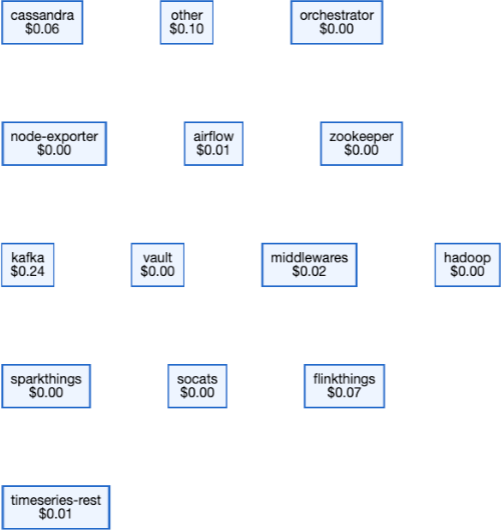
\includegraphics[width=\textwidth]{gfx/sb-cost.png}
    \caption{Cost per service of the Sustainability Buildings Company for one hour}
    \label{fig:sb-cost}
\end{figure}

\noindent
This computation is based on the equation described in \autoref{eq:p}. By using this formula, it is also interesting to see the distribution of the CPU usage and memory usage. This is shown in \autoref{fig:sb-cost-cpu} and \autoref{sb-cost-mem}. Lastly, the waste distribution shows which services are responsible for the most waste cost. This is shown in \autoref{fig:sb-waste}.

\begin{figure}
    \centering
    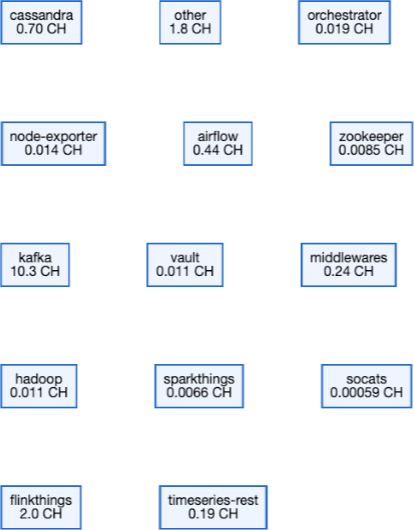
\includegraphics[width=\textwidth]{gfx/sb-cost-cpu.png}
    \caption{CPU usage cost per service of the Sustainability Buildings Company for one hour}
    \label{fig:sb-cost-cpu}
\end{figure}

\begin{figure}
    \centering
    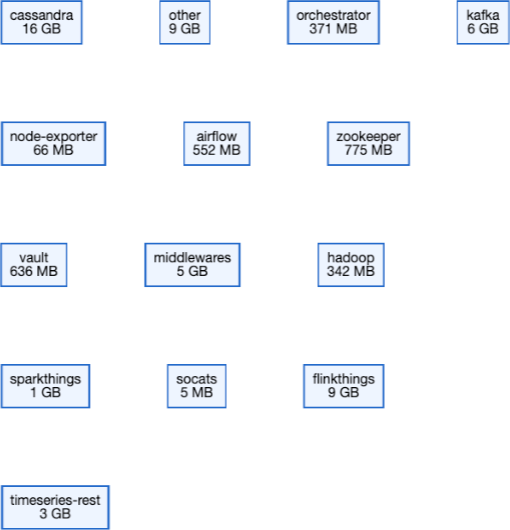
\includegraphics[width=\textwidth]{gfx/sb-cost-mem.png}
    \caption{Memory usage cost per service of the Sustainability Buildings Company for one hour}
    \label{fig:sb-cost-mem}
\end{figure}

\begin{figure}
    \centering
    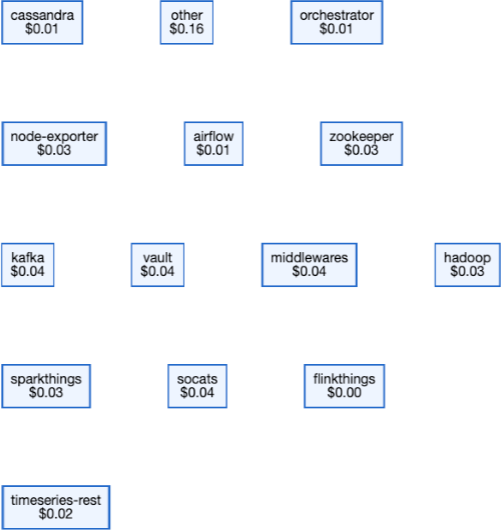
\includegraphics[width=\textwidth]{gfx/sb-waste.png}
    \caption{Waste cost per service of the Sustainability Buildings Company for one hour}
    \label{fig:sb-waste}
\end{figure}

\section{Limitation} \label{sec:sb-limitation}
The system proposed in \autoref{ch:design} is able to monitor the CPU and memory usage on a container level. Using TCPDump, a subsampling procedure has been implemented that monitors the packets on a host level. Then, the system assigns this packets to a container by resolving their IP address. However, almost all their communication of their services are configured using Weave Net\footnote{See \url{https://github.com/weaveworks/weave}}. Weave Net creates a virtual network that connects Docker containers across multiple hosts and enables their automatic discovery. To application containers, the network established by Weave resembles a giant Ethernet switch, where all containers are connected and can easily access services from one another. \cite{weave}.\\

\noindent
When using the weave network, the containers don't communicate by their exposed IP address. Therefore, the proposed system is unable to resolve the internet packets. This leads to a lower estimate of $n_\text{internal}$ in \autoref{formula:traffic}, which results in a higher $n_\text{network}$. Therefore, the estimated cost using \autoref{eq:p} is also too high. Further work is needed to resolve the IP addresses according to the weave network.


\section{Conclusion} \label{sec:sb-evaluation}
In order to evaluate the deployment of the system, the decision has been made to perform an interview with one of the employees of the company. The entire interview can be found in \autoref{ch:interview}. From this interview it can be concluded that ....\\

\noindent
For the reproducibility of the case study, the data has been made publicly available\footnote{Get the data from \url{https://drive.google.com/file/d/1SUy_j3WpSjCaZ54KeotaE4xhF87rrjwh/view?usp=sharing}}. This file is the compressed data folder from the Prometheus database. This can therefore be used to generate the visualizations above.